\section{Latin Square Study}\label{sec:s02}

This study uses a different experimental design that makes it possible to control for the experience of the subjects. It employs a subset of the atom candidates used in the repeated measures study. More specifically, this study investigates ten of the atoms investigated in the repeated measures study: 
%Since JavaScript and \clang have some constructs in common (Section~\ref{back}), we first 
%select a set of 9+1 atom candidates: 
nine previously-validated atoms of confusion for the \clang language~\cite{DBLP:conf/sigsoft/GopsteinIYDZYC17} that also exist in JavaScript programs plus one atom candidate that is specific to the JavaScript language (Automatic Semicolon Insertion).  
%Our supplementary material discusses and shows examples of the atoms we consider in our research.\castor{We should probably do this here or just refer to the table that I intend to insert for the replication study.}

\subsection{Experimental design} 

The design of the Latin square study blocks two variables (subject experience and the programs) and considers two treatments: the presence or absence of atom candidates within the programs. To achieve such a design goal, controlling the effect of experience and individual programs, we resort to the \textit{Latin Square Design}~\cite{Hunter-Experimenters}. Using this design we create a 2 x 2 matrix in which each row represents a subject and each column indicates the set of programs. The design of each square (a replica) is such that no treatment is repeated in the same row or column. For example, considering that we have a set of 10
code samples $s_0, s_1, ..., s_{10}$, if a given subject (P1) is asked to predict the output of the code samples $s_0, s_1, ..., s_5$ that contain atom candidates, then, when answering questions about clean programs, they will only be presented with clean versions of the code samples $s_6, s_7,..., s_{10}$. Furthermore, a given subject (P2), who constitutes the second row of our example square, will be asked questions about the clean versions for $s_1, s_2, ..., s_5$, and will answer questions about obfuscated programs for $s_6, s_7,..., s_{10}$. By doing that, we guarantee that all versions of the programs are contained within each square, and that each configuration occurs only once within a square. Figure \ref{fig:latinsquare} offers a visual representation of the concept.

  \begin{figure}[htb!]
      \noindent
      \centering
      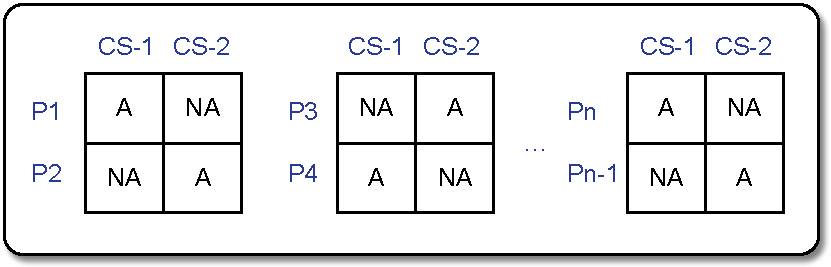
\includegraphics[scale=.50]{images/latin-square.pdf}
      \caption{Latin square design. Each ``square'' corresponds to 
      a replica in our study. Each replica comprises two participants (square rows, e.g., P1 and P2) 
      and two sets of programs (CS-1 and CS-2). We randomly apply the 
      treatments (atom or non-atom code) to the cells of the squares.} 
      \label{fig:latinsquare}
  \end{figure}

For each of the 10 selected atom candidates, we write one short program containing the atom. As in the repeated measures study, we call them the obfuscated versions of the programs. We also write corresponding short programs without the atom candidates and call them the clean versions of the programs. Overall, the experiment employed 20 programs, 10 obfuscated and 10 clean. In order to reduce the cognitive effort, each subject was asked to predict the output of 10 programs, five obfuscated and five clean. The order in which they are presented is randomized. By doing this, we seek to minimize the chances of subjects being aware that the current listing they are analyzing contains (or not) atoms of confusion. That is, each subject should indicate what would be the outcomes of the programs, some of them having atoms of confusion (while other programs do not). Since participants are not exposed to obfuscated and clean versions corresponding to the same atom candidate, learning effect is not possible. We measure answer correctness and the total time each participant requires to participate in the experiment.

{\bf Study instrument.} 
We implemented our experiment as a questionnaire in a web application and 
%carried out a pilot. 
%As part of this effort, we 
carried out an informal pilot. Undergraduate students and professional colleagues took part in the pilot. Some users reported layout defects, and many reported that the landing page did not explain the study well enough. We also spotted minor issues with our routines to create and populate the latin squares. 

We organize the questionnaire in three sections. The first section aims to characterize the subjects, asking their age, education level, and programming experience. We also include a check button, whose checking means users agree that all collected data will be used solely for research purposes. In the second section, we present to the participants a small set of instructions, where we explain how the study works and ask them to dedicate their attention to it. We stress to participants the importance of not using any aids during the experiment, such as online or console interpreters. For each question page, we kept track of whether or not the subjects switch windows. 

The last section of the questionnaire presents a sequence of ten questions, each containing a program. For each question, there is a text box where the answer should be written. There is also an ``I do not know'' button, which, when clicked, leads the subject to the next question. In our setting, ``I do not know'' is treated as a wrong answer. The programs are also presented as images copied from a text editor. Upon submitting their answer for a particular question, the subjects are automatically led to a similar page, containing another program. Similarly to the repeated measures study, we do not provide feedback about time and correctness to the subjects.


% \rb{nao acho esse paragrafo necessario} 
% \adriano{o de baixo ne? eu tambem acho}

% As we mentioned before, we first wrote the code listings in a text editor, and took pictures of it. In the case of an atom of confusion that was exclusive to JavaScript, which we called \textit{Automatic Semicolon Insertion} (see Appendix~\ref{sec:appendix-atoms}), it was necessary to remove the syntax highlighter. Even though semicolons at the end of statements are optional to programmers in JavaScript, the interpreter automatically inserts them into the code. Our text editor was incorrectly highlighting a line break after a return statement, even thought it was valid JavaScript syntax. We had thus to turn the highlighter off to take the picture of this atom. 

{\bf Study audience.}
We posted the invitation to take part in the study on a JavaScript Reddit channel.\footnote{https://www.reddit.com/r/javascript/} We explained our research purposes and asked developers of any level of expertise to take part. Within twelve hours, we collected more than 150 answers, populating more than 70 replicas of the Latin Squares. We collected significant data on time taken and discrepancies in answer correctness between obfuscated and clean versions of the programs. Some inconsistencies arose while building the squares, for instance, when a user quit in the middle of the questionnaire. We discarded from our study all squares that contained incomplete rows.

%Since we had a large enough number of samples, the squares we had to discard did not impact our analysis.

\subsection{Results}\label{sec:latin}

In the latin-square study, we estimate the impact of atoms considering the same two perspectives of the previous experiment: \emph{correctness} (number of wrong answers)
and \emph{time} (how long to provide a correct answer). In particular, in the time analysis, differently from the repeated  measures study, we compare the time required by participants to submit a correct response when analyzing code snippets with and without atom candidates. This study is based on the responses of 140 participants (a total of 70 replicas). All participants had taken at least some university course or hold a bachelor degree or equivalent. In addition, 21 participants hold a master's degree and three a doctorate degree. Considering the programming experience of our respondents, 19\% have more than ten years of programming experience, 37\% have between four and ten years of experience, 37\% have between one and four years of experience, and 7\% have less than one year of programming experience.  
Accordingly, we characterize the effect of atoms of confusion in JavaScript code taking into account the perceptions of both novice and experienced developers. 

\subsubsection{Correctness Analysis}
% \castor{We need to be uniform about terminology. Are we going with ``misunderstanding rate analysis''? The problem is that it is not clear to me to which rate this refers.}

{\bf Exploratory Data Analysis.}
As mentioned in Section~\ref{sec:meth:survey}, each participant in this experiment evaluated ten code snippets, from which five were in their obfuscated versions, whilst the other five contained clean versions of the code snippets (i.e., without the atom candidates). As in the repeated measures study, the participants should provide the expected outcomes of the code snippets. Differently from that study, in this one each participant only predicts the outcome of one version of each code snippet, either clean or obfuscated. As discussed, we collect information about \emph{correctness} (whether the participant correctly predicted the program's output) and \emph{time}. 
Table~\ref{tab:difference-correctness} and Figure~\ref{fig:boxplotcorrectness} summarize the results of the correctness experiment.

Considering Table~\ref{tab:difference-correctness}, the clean versions of six code snippets present at least a 15\% improvement in answer correctness when compared with the obfuscated versions. In particular, the presence of the \emph{Comma Operator} atom exhibits the highest impact on misunderstanding. 
Frequently used constructs and idioms, such as \emph{Post Increment} and \emph{Omitted Curly Braces} (see Section~\ref{sec:msr-results}), also result in many mistakes. %introduce high degrees of confusion.
The boxplot of Figure~\ref{fig:boxplotcorrectness} shows a non-negligible decrease in the average number of incorrect answers when observing the clean versions of the code snippets. Also, the sample of responses with no atoms had almost no dispersion, which supports the argument that the clean versions of the code snippets are easier to evaluate correctly. 


% \begin{table}[htbp]
% \caption{Difference in answer correctness between confusing and non-confusing pairs}
% \begin{center}
% \begin{small}
% \begin{tabularx}
% {{\linewidth}}{l p{1.5cm} p{1.1cm} p{1.1cm} p{1.2cm} }
% \textbf{Atom} & \textbf{\%Correct} & \textbf{\%Correct} \\
% &  \multicolumn{1}{l}{With AOC} \multicolumn{2}{l}{Without AOC}  & \Delta (\%)    \\
%  \hline
% Comma Operator & 40 & 93 & +132\%                 \\     
% Automatic Semicolon  Insertion & 46 & 97 & +110\% \\
% Post Increment & 69 & 91 & +31\%         \\
% Omitted Curly Braces & 67 & 83 & +23\%   \\ 
% Assignment as Value & 80 & 97 & +21\%    \\
% Implicit Predicate & 83 & 97 & +16\%     \\
% Logic as Control Flow & 59 & 68 & +15\%  \\
% Ternary Operator & 86 & 94 & +9\%        \\
% Pre-Increment & 71 & 76 & +7\%           \\
% Arithmetic as Logic & 91 & 90 & -1\%    \\
% \end{tabularx}
% \end{small}
% \end{center}
% \label{results_correctness}
% \end{table}

\begin{table}[htbp]
\caption{Summary of the correctness analysis}
\label{tab:difference-correctness}
\centering{
  {\scriptsize
  \begin{scriptsize}
\begin{tabular}{lrrr} \toprule
  Atom & Obfuscated & Clean & $\Delta$(\%)  \\ \midrule
  Comma Operator                &  28 &  65 & +132   \\ 
  Automatic Semicolon Insertion &  32 &  68 & +112   \\ 
  Post-Increment                &  48 &  64 & +33    \\ 
  Omitted Curly Braces          &  47 &  58 &  +23   \\
  Assignment as Value           &  56 &  68 &  +21   \\ 
  Implicit Predicate            &  58 &  68 &  +17   \\ 
  Logic as Control Flow         &  41 &  48 &  +17   \\ 
  Conditional Operator              &  60 &  66 &  +10   \\ 
  Pre-Increment                 &  50 &  53 &  +6    \\ 
  Arithmetic as Logic           &  64 &  63 &  -2    \\ \bottomrule
  
\end{tabular}
\end{scriptsize}
}}
\end{table}

 %% Comma Operator          & 40 & 93  & +132 \\
 %% Post Increment          & 69 & 91  & + 31  \\
 %% Omitted Curly Braces    & 67 & 83  & +23 \\
 %% Assignment as Value     & 80 & 97  & +21 \\
 %% Implicit Predicate      & 83 & 97  & +16 \\
 %% Logic as Control Flow   & 59 & 68  & +15 \\
 %% Ternary Operator        & 86 & 94  & +9  \\
 %% Pre-Increment           & 71 & 76  & +7  \\
 %% Arithmetic as Logic     & 91 & 90  & +1  \\ \bottomrule


\begin{figure}[b!]
\noindent
 \centering
 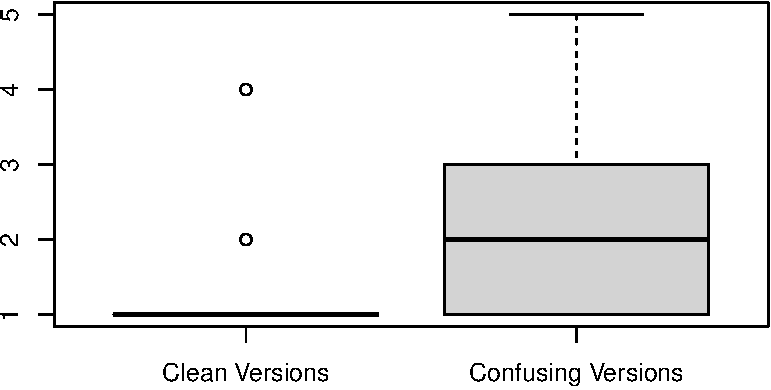
\includegraphics[width=0.6\columnwidth]{images/wrong-answers-plot-1.pdf}
 \caption{Number of wrong answers of each subject.}
 \label{fig:boxplotcorrectness}
 \end{figure}% \castor{Fiz de tudo para ajeitar a figura porque o texto embaixo deveria ser "Clean versions" e "Confusing versions" mas não sei porque não funcionou. Até mudei a figura. Não sei o que está havendo.}
 
% \rb{verificar a consistencia nas questoes de pesquisa mais especificas}

{\bf Statistical analysis.}
We first use the \emph{Pearson's Chi-squared test}
to investigate if there is a statistically significant difference in the frequency of correct and incorrect answers---due to the versions of the code snippets (obfuscated and clean code). The p-values for these tests are reported in the ``Chi-square test'' column of Table~\ref{tab:hypothesis-testing}. For five atom candidates (Comma Operator, Automatic Semicolon Insertion, Post-Increment, Assignment as Value, Implicit Predicate), the results indicate that the obfuscated versions of the code snippets have a negative impact on code understanding (p-value $< 0.05$). This result holds even after applying the Benjamini-Hochberg correction with a false discovery rate of 5\%. 

We measure the effect size of the clean version of the code snippets into the answers' correctness using the \emph{Odds Ratio} (OR). The results are reported in the ``Odds Ratio'' column of Table~\ref{tab:hypothesis-testing}. 
In the table, we also report the confidence interval (CI) for the OR in the ``CI'' column. Although many of the intervals are wide, for six of the atom candidates the lower bound of the confidence interval is greater than or equal to 1. This indicates that, at a 95\% confidence level, a developer is likely to commit less mistakes when using the clean versions. 
%Considering only the atoms for which there was a significant difference in correctness for confusing and clean versions and u
%Using the thresholds established by Chen and colleagues~\cite{Chen:2010:HBB} (OR = 1.68 small, 3.47 medium, and 6.71 large), 
For four of the atoms, Comma Operator, Automatic Semicolon Insertion, Assignment as Value, and Implicit Predicate, effect size can be considered large. For Implicit Predicate, it is medium. 
%We found a negligible effect size for the atom candidates Arithmetic as Logic, Logic as Control Flow, and Pre-Increment. Nonetheless, for the remaining candidates, the effect size is significant. 
For instance, when comparing clean and obfuscated code snippets pertaining to the Comma Operator atom candidate, we observed an \emph{Odds Ratio} of \num{19.02}. This means that the odds of a correct answer are \num{19.02} times higher when interpreting the clean version---in comparison with the corresponding obfuscated version of the code snippet. Furthermore, with a 95\% confidence level, the odds ratio is between 6.6 and 68.22, i.e., although the error margin is wide, it is strongly in favor of the clean version. If there is a significant likelihood of a developer committing a mistake when analyzing a clean version, the lower bound of the CI should be a number between 0 and 1 (since the OR is a ratio). This is the case for the four atom candidates in the lower part of the table. 
%In particular, in the last row (Arithmetic as Logic), the OR between 0 and 1 indicates that a participant was actually more likely to misunderstand the clean version. 

Finally, we also use a \emph{Binomial Generalized Logistic Regression} analysis to investigate if either \emph{participant education} or \emph{participant experience} impacts correctness. The findings suggest that \emph{participant experience} impacts the results related to correctness (p-value $<$ 0.001 and $\chi^2 = 24.18$).
Figure~\ref{fig:correctness-over-experience} summarizes the number of correct and incorrect answers over the four experience groups. Even though the presence of atoms of confusion reduces the number of correct answers for all \emph{experience groups}, this effect is not uniform. For instance, novice developers (under one year of experience) provide a higher number of wrong answers for the obfuscated version of the code (57.8\%), while developers with more than four years of experience provide more than 70\% of correct answers even when evaluating the obfuscated version of the code snippets. It is also important to note that, independently of the \emph{experience group}, developers tend to provide more than 84\% of correct answers while predicting the outputs for the clean versions of the code. We replicate the \emph{Pearson's Chi-squared test} for each experience group and find that the statistical difference is less significant for those developers with more than ten years of experience (p-value = 0.007 and $\chi^2$ = 7.08). Differently from \emph{participant experience}, the factor \emph{participant education} does not significantly change the correctness of the answers (p-value = 0.236 and $\chi^2$ = 5.54).

% \castor{I'd like to have the numbers for the results above. What are the p-values, regression coefficients, etc.?}

\begin{figure}
  \centering
  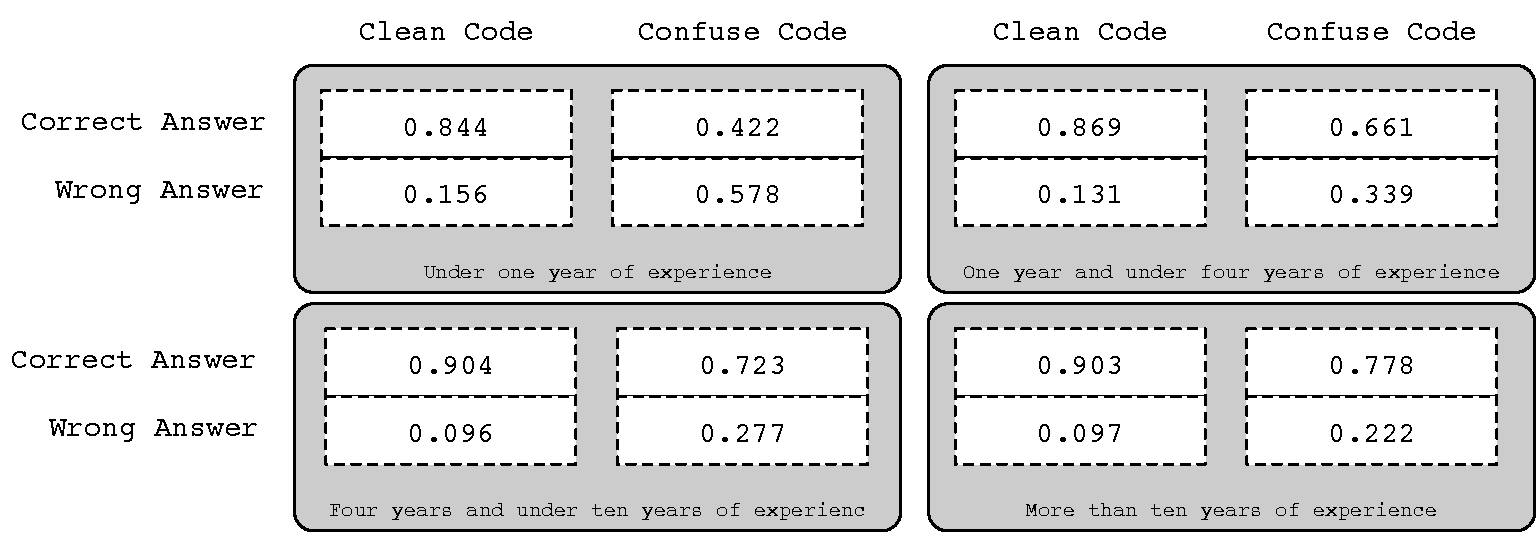
\includegraphics[scale=0.5]{images/correctness-by-experience}
  \caption{Impact of atoms of confusion on the correctness (over the four participant experience groups)}
  \label{fig:correctness-over-experience}
\end{figure}


%% \begin{mh}
%%   The results of our exploratory data analysis and   hypothesis testing suggest that the atom candidates Comma Operator, Automatic Semicolon Insertion, Post Increment, Omitted Curly Braces, Assignment as Value, and Implicit Predicate %, and Ternary Operator
%%   introduce some degree of misunderstanding in JavaScript code. %Based on the results of this study, 
%%   Therefore, they can be deemed atoms of confusion for JavaScript.
%% \end{mh}

%% \begin{mh}
%% {\color{red}Comparing the results of different studies,
%%   the impact of atoms candidates on source code
%%   (mis)understanding differ according to the programming
%%   language.}
%% \end{mh}
%% Regarding the first question we 
%% address in the survey (\emph{Do code snippets that contain atoms of confusion produce a higher error rate than snippets where the atom is removed?}), we found evidence that the atoms of confusion lead programmers to misunderstand JavaScript code. We also realized that just one atom whose correction has a non-significant improvement in the percentage of correct answers---we found an improvement of at least 15\% in the correct answers when removing the confusing code for seven atoms (out of ten atoms we consider in the survey). 

\subsubsection{Time Analysis}

{\bf Exploratory Data Analysis.}
Table \ref{tab:difference-time-taken} shows the average time necessary for the participants to give a correct answer about the expected outcomes of a code snippet, considering both obfuscated and clean versions. We do not consider cases where the participants made mistakes. Seven atom candidates required more time from participants to predict a correct response. For these eight atom candidates, developers take at least 5.90\% less time on average to find a correct answer when considering the clean version of a code snippet. In the extreme case (atom candidate Comma Operator), the participants take 76.23\% less
time on average to find the correct answer for the clean version of the code snippets. 
Not all atom candidates, though, require less time for the participants to predict the answer. In fact, for  Arithmetic as Logic and Pre-Increment, the time to give a correct answer for the clean versions was   
29.06\% and 38.19\% smaller than for the obfuscated versions---we did not confirm these atom candidates as atoms of confusion in the previous section.

\begin{table}[htbp]
\caption{Time in seconds to submit a correct answer}
\centering{
  {\scriptsize
  \begin{scriptsize}
\begin{tabular}{lrrr} \toprule
Atom & Obfuscated  & Clean & $\Delta$(\%) \\ \midrule
Comma Operator & 87.67 & 20.84 & -76.23 \\ 
Automatic Semicolon Insertion & 46.08 & 22.04 & -52.17 \\ 
Post-Increment & 28.70 & 25.67 & -10.56 \\ 
Omitted Curly Braces & 48.85 & 30.00 & -38.58 \\ 
Assignment as Value & 52.47 & 48.95 & -6.71 \\ 
Implicit Predicate & 36.24 & 24.01 & -33.75 \\ 
Logic as Control Flow & 108.94 & 51.07 & -53.12 \\ 
Conditional Operator & 41.80 & 39.34 & -5.90 \\ 
Pre-Increment & 30.71 & 42.45 & 38.19 \\  
Arithmetic as Logic & 28.82 & 37.20 & 29.06 \\ \bottomrule
\end{tabular}
\label{tab:difference-time-taken}
\end{scriptsize}
}}
\end{table}

 % latex table generated in R 4.0.4 by xtable 1.8-4 package
 % Thu Apr 22 07:58:21 2021
 \begin{table*}[ht]
\caption{Hypotheses Testing (misunderstanding and time). Asterisks ($^{*}$) indicate a statistically significant difference.}
 \centering
 {\scriptsize
 \begin{tabular}{lrrr|rr}
   \toprule
      & \multicolumn{3}{c}{Correctness analysis} & \multicolumn{2}{c}{Time analysis} \\ \toprule
Atom  & Chi-square & Odds           & Confidence & Mann-Whitey& Cliff's\\ 
 &  test &Ratio          & Interval &  U test & Delta \\  \midrule
Comma Operator & \textbf{$<$ 0.0001*} & 19.02 & (6.60, 68.22) & \textbf{$<$ 0.0001*} & -0.53 \\ 
Automatic Semicolon Insertion & \textbf{$<$ 0.0001*} & 39.33 & (9.21, 356.62) & 0.0980 & -0.16 \\ 
Post-Increment & \textbf{0.0015*} & 4.83 & (1.73, 15.74) & 0.1201 & 0.15 \\ 
Omitted Curly Braces & 0.0510 & 2.35 & (1.00, 5.77) & 0.9253 & -0.01 \\ 
Assignment as Value & \textbf{0.0035*} & 8.39 & (1.81, 79.12) & 0.8268 & 0.02 \\ 
Implicit Predicate & \textbf{0.0112*} & 6.95 & (1.46, 66.56) & \textbf{0.0029*} & -0.29 \\ 
Logic as Control Flow & 0.2920 & 1.54 & (0.73, 3.28) & \textbf{$<$ 0.0001*} & -0.39 \\ 
Conditional Operator & 0.1590 & 2.73 & (0.74, 12.57) & 0.2407 & -0.12 \\ 
Pre-Increment & 0.7015 & 1.25 & (0.55, 2.85) & \textbf{0.0062*} & 0.27 \\ 
Arithmetic as Logic & 1 & 0.84 & (0.22, 3.12) & \textbf{0.0172*} & 0.23 \\ 
    \bottomrule
 \end{tabular}}
 \label{tab:hypothesis-testing}
 \end{table*}


{\bf Statistical analysis}
We use the \emph{Mann-Whitney U test} to
investigate the null hypothesis that developers 
spend the same amount of time to correctly
predict the outcome of clean and obfuscated versions of a code snippet.
%, regardless of evaluating the confusing or clean version of the code.
The results of Table~\ref{tab:hypothesis-testing}
suggest that we should refute the null hypotheses for five atom candidates (Comma Operator, Implicit Predicate, Logic as Control Flow, Pre-Increment, and Arithmetic as Logic), after applying the Benjamini-Hochberg correction with a false discovery rate of 5\%. For the first three, the analysis suggests that the participants need more time to predict the outcome of the code snippet in the obfuscated code version. For the atom candidates Arithmetic as Logic and Pre-Increment, the participants take less time to predict the outcome of the code snippets in the obfuscated version. We also computed the effect size using Cliff's Delta statistic. In the table, negative effect sizes suggest that it took less time to correctly predict the output of clean versions of the snippets.  Considering the thresholds established by Romano et al.~\cite{Romano:2006:ASO} (0.147 $<$ $|$d$|$ $<$ 0.33 small, $|$d$|$ $<$ 0.474 medium, otherwise large), we found a large effect for the Comma Operator atom candidate; a medium effect size for Logic as Control Flow, and small effect sizes for Automatic Semicolon Insertion, Implicit Predicate, Arithmetic as Logic, Post-, and Pre-Increment. 


%% \begin{mh}
%%   The results suggest that developers tend to spend
%%   more time to predict the correct answer in the presence of the atom candidates Comma Operator, Logic as Control Flow, and Implicit Predicate. Conversely, the code snippets with the atom candidates Arithmetic as Logic and Pre-Increment demand less time to predict the correct answers. 
%% \end{mh}


%%  Comma Operator        & 60 & 21  & -65  \\
%% Logic as Control Flow & 85 & 49  & -42  \\
%% Implicit Predicate    & 33 & 24  & -27  \\
%% Omitted Curly Braces  & 43 & 31  & -27  \\
%% Assignment as Value   & 53 & 49  & -7   \\
%% Ternary Operator      & 42 & 42  & 0    \\
%% Post Increment        & 27 & 27  & 0    \\
%% Arithmetic as Logic   & 29 & 36  & +24  \\
%% Pre-Increment         & 34 & 49  & +44  \\


% \rb{acho que podemos melhorar a apresenta\c c\~{a}o dessas tabelas, talvez usando booktabs.}


